\section{Executable Context-Budget Probe}

\begin{table*}[t]
\centering
\small
\caption{Summary of the executable serialization probe on 240 synthetic 16$^3$ microenvironments (average occupancy 107.6 voxels). Lower neighbor span is better. Higher retention and recoverability are better.}
\label{tab:probe-summary}
\resizebox{\textwidth}{!}{%
\begin{tabular}{lrrrrrrr}
\toprule
Ordering & Mean 6-neighbor span & Median 6-neighbor span & Adj. $\leq 8$ & Adj. $\leq 16$ & Recover $\leq 128$ & Recover $\leq 256$ & Recover $\leq 512$ \\
\midrule
Hilbert & 149.9 & 5 & 0.598 & 0.652 & 0.486 & 0.595 & 0.718 \\
Morton & 139.2 & 4 & 0.572 & 0.645 & 0.448 & 0.586 & 0.704 \\
Raster & 91.2 & 16 & 0.333 & 0.666 & 0.029 & 0.313 & 1.000 \\
Random & 1352.4 & 1181 & 0.003 & 0.006 & 0.000 & 0.002 & 0.016 \\
\bottomrule
\end{tabular}
}
\end{table*}

\begin{figure}[t]
\centering
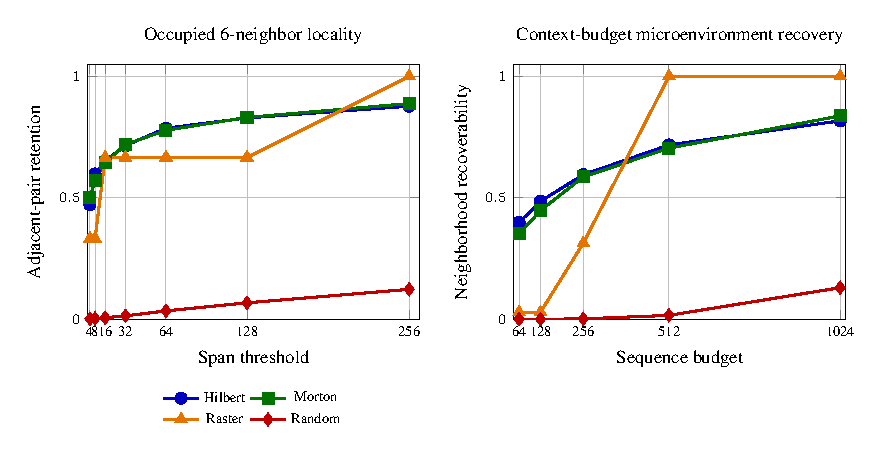
\includegraphics[width=0.98\linewidth]{../figure_assets/probe_curves/probe_curves.pdf}
\caption{Computed probe curves. Left: retention of occupied 6-neighbor pairs as the allowable serialized span increases. Right: recovery of mixed-channel local environments as the available sequence budget increases. Hilbert and Morton behave smoothly under tight budgets, raster shows a plane-boundary cliff, and random order destroys locality.}
\label{fig:probe-curves}
\end{figure}


A purely conceptual upgrade would still invite a reasonable reviewer objection: if serialization truly matters as an interface, can the claim be made operational in a small, reproducible study? To answer that question without inventing a fake biomolecular benchmark, we add a deterministic synthetic probe that isolates the paper's central design variable.

The probe builds 240 voxelized 16$^3$ microenvironments with three semantic channels. Each sample combines backbone-like walks, dense pocket-like patches, and distractor voxels, yielding an average occupancy of 107.5 voxels. The goal is not biological realism or state-of-the-art prediction. The goal is narrower and better aligned with the paper's thesis: measure how an ordering changes which local structural evidence becomes visible to a bounded-context sequence processor.

We compare four serializations: Hilbert, Morton, raster scan, and a random control. Two metrics are reported. The first is occupied 6-neighbor locality: for every adjacent occupied voxel pair, we measure the 1D span induced by the ordering. The second is neighborhood recoverability: for every center voxel whose 3D neighborhood contains at least one channel-1 neighbor, two channel-2 neighbors, and two channel-3 neighbors, we compute the smallest sequence radius that exposes the required supporting voxels. This gives a direct context-budget diagnostic for sequence-native models.

The results support the upgraded thesis. Hilbert retains 59.8\% of occupied 6-neighbor pairs within span 8, compared with 33.3\% for raster and 0.3\% for random. Morton is competitive at 57.2\%, which is useful rather than inconvenient: the result suggests that locality-aware serialization is the important family-level idea, not that one historical curve is magically dominant in every regime. The more revealing metric is neighborhood recoverability. At a sequence budget of 128 tokens, Hilbert recovers 48.6\% of positive local environments, Morton 44.8\%, raster 2.9\%, and random effectively zero. At 256 tokens, Hilbert reaches 59.5\%, Morton 58.6\%, raster 31.3\%, and random 0.2\%. Raster only catches up when the budget exceeds its plane-boundary cliff at 512 tokens, a reminder that average span alone can hide brittle worst-case behavior.

This probe does not prove biomolecular superiority, but it does provide the missing empirical bridge between the 2018 intuition and the modern interface claim. The key message is that serialization quality becomes most visible under constrained context budgets, which is exactly the regime where sequence-native backbones become attractive.
